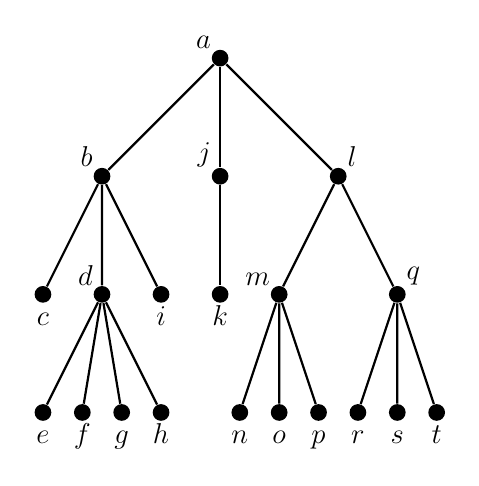
\begin{tikzpicture}[thick,scale=0.5, every node/.style={scale=0.5}, level distance=3cm]
    \tikzstyle{marrs}=[very thick,-latex]
    \tikzstyle{tnode}=[circle, fill=black, inner sep=1.5mm]
    \def\rstep{5cm}
    
    \huge
    
    \tikzstyle{level 1}=[sibling distance=3cm]
    \tikzstyle{level 2}=[sibling distance=1.5cm]
    \tikzstyle{level 3}=[sibling distance=1cm]
    
    \node[tnode] (a) {}
        child { node[tnode] (b) {} 
            child { node[tnode] (c) {} }
            child { node[tnode] (d) {} 
                child { node[tnode] (e) {} }
                child { node[tnode] (f) {} }
                child { node[tnode] (g) {} }
                child { node[tnode] (h) {} }
            }
            child { node[tnode] (i) {} }
        }
        child { 
            node[tnode] (j) {} 
            child { node[tnode] (k) {} }
        }
        child { node[tnode] (l) {} 
            child { node[tnode] (m) {} 
                child { node[tnode] (n) {} }
                child { node[tnode] (o) {} }
                child { node[tnode] (p) {} }
            }
            child[missing] {}
            child { node[tnode] (q) {} 
                child { node[tnode] (r) {} }
                child { node[tnode] (s) {} }
                child { node[tnode] (t) {} }
            }
        }
    ;
    \foreach \i in {c, e, f, g, h, i, k, n, o, p, r, s, t} {
        \node[below=8mm, anchor=base] at (\i) {$\i$};
    }
    \foreach \i in {a, b, d, j, m} {
        \node[above left] at (\i) {$\i$};
    }
    \foreach \i in {l, q} {
        \node[above right] at (\i) {$\i$};
    }
    
    
    
\end{tikzpicture}